\subsection{Drei spezialisierte Visualisierungssysteme}

M.A.S.K. implementiert drei spezialisierte Visualisierungssysteme, die über eine gemeinsame Infrarot-Tracking-Pipeline gesteuert werden. Die Architektur folgt einem modularen Ansatz, bei dem jede Komponente eigenständig funktioniert und über standardisierte Schnittstellen kommuniziert.

\textbf{Visual-System 1: Hand-Feuer-Effekte}

\begin{figure}[h]
    \centering
    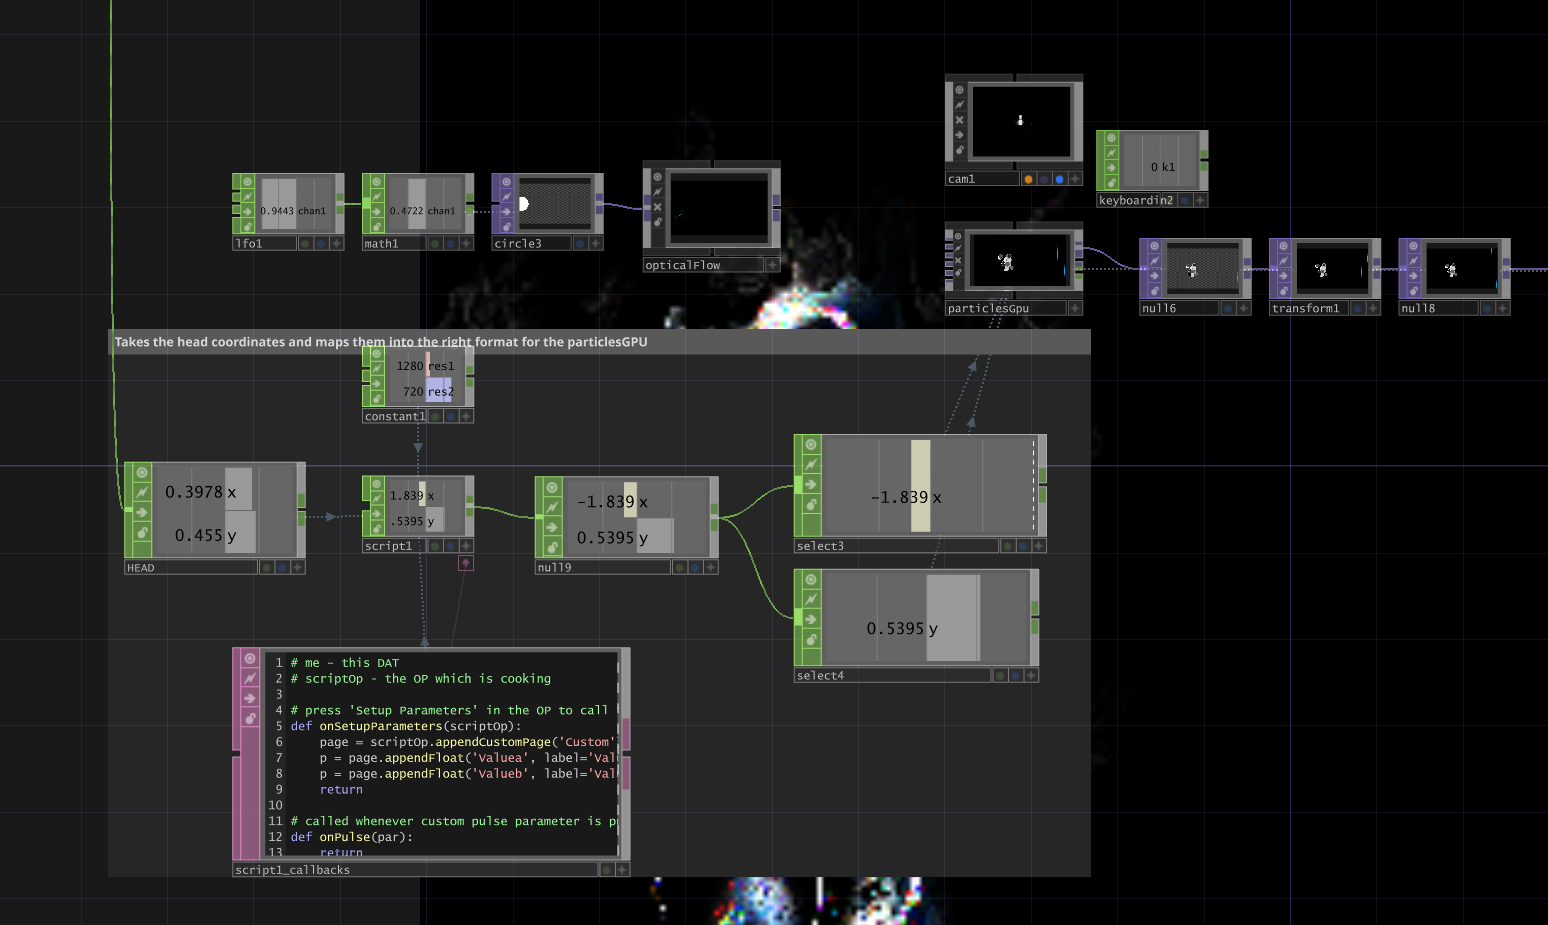
\includegraphics[width=0.9\textwidth]{images/docupictures/NoisyBlob_HEAD_to_ParticleGPU_Translate.png}
    \caption{Hand-Feuer-Effekte: Blaue Partikel folgen Handbewegungen in Echtzeit}
    \label{fig:particle_hands}
\end{figure}

Das Hand-Feuer-System nutzt TouchDesigners ParticleGPU für die Erzeugung blauer Flammenpartikel. Die Implementation extrahiert Hand-Node-Positionen aus MediaPipe (Wrist-Landmarks 15 und 16) und transformiert diese in normalisierte Bildschirmkoordinaten. Die Partikel-Emission erfolgt geschwindigkeitsabhängig mit einer Lebenszeit von 1,2 Sekunden.

\textbf{Visual-System 2: Adaptive Kopfpartikel}

\begin{figure}[h]
    \centering
    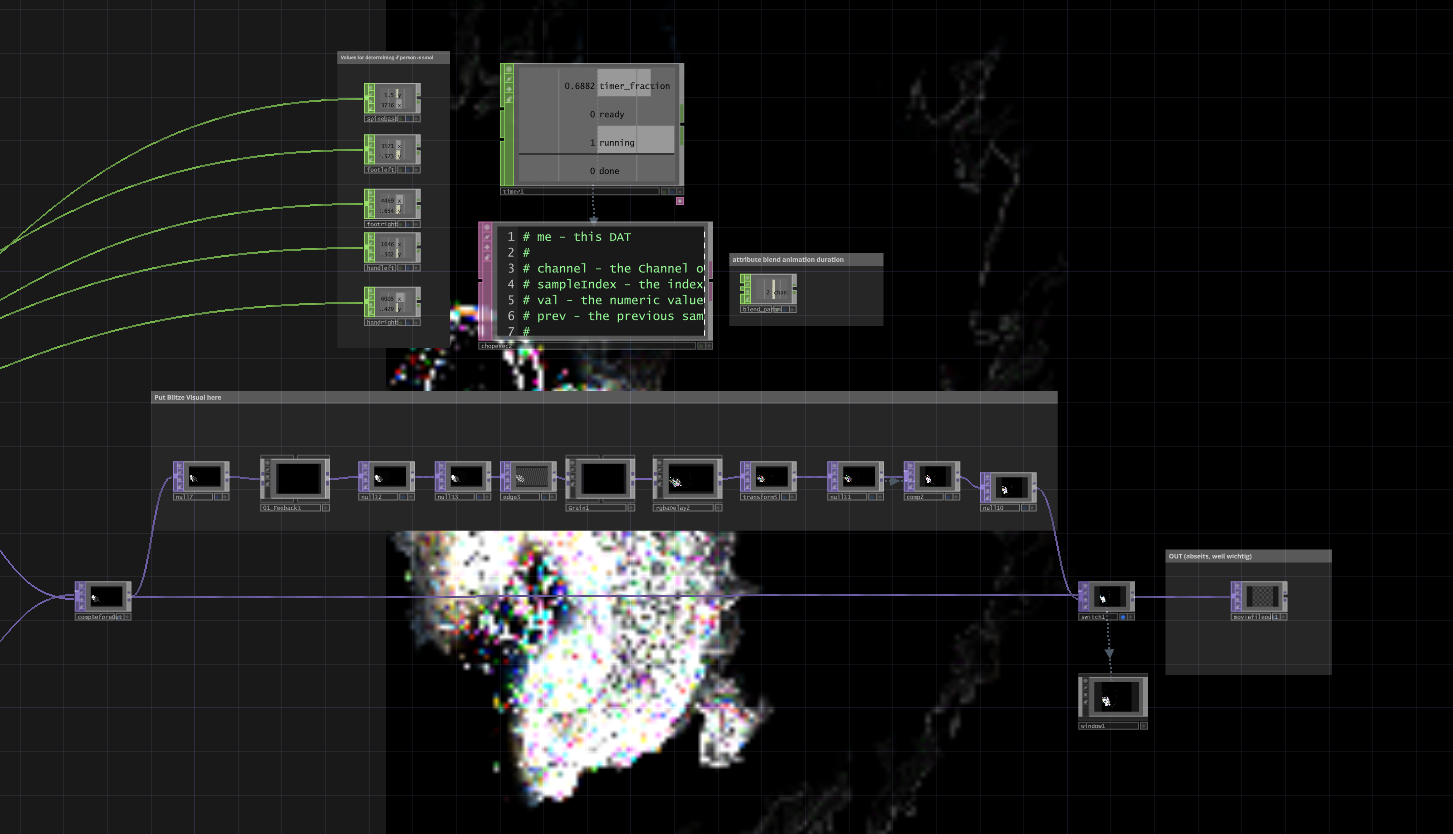
\includegraphics[width=0.9\textwidth]{images/docupictures/NoisyBlob_animatedSwitchzwischenBlitzUndNichtBlitzBeiTrackingTrigger.png}
    \caption{Adaptive Kopfpartikel: Zustandswechsel basierend auf Handposition relativ zur Schulter}
    \label{fig:relative_switch}
\end{figure}

Die Kopfpartikel-Implementation verwendet eine Zustandsmaschine mit zwei Modi. Der Wechsel erfolgt durch Vergleich der Y-Koordinaten von Hand- und Schulter-Nodes. Eine Interpolationsfunktion sorgt für sanfte Übergänge zwischen den Zuständen. Die frontale Ausrichtung erfordert präzise Kalibrierung der Beamer-Kamera-Relation.

\textbf{Visual-System 3: 64-Spike Radialsystem}

\begin{figure}[h]
    \centering
    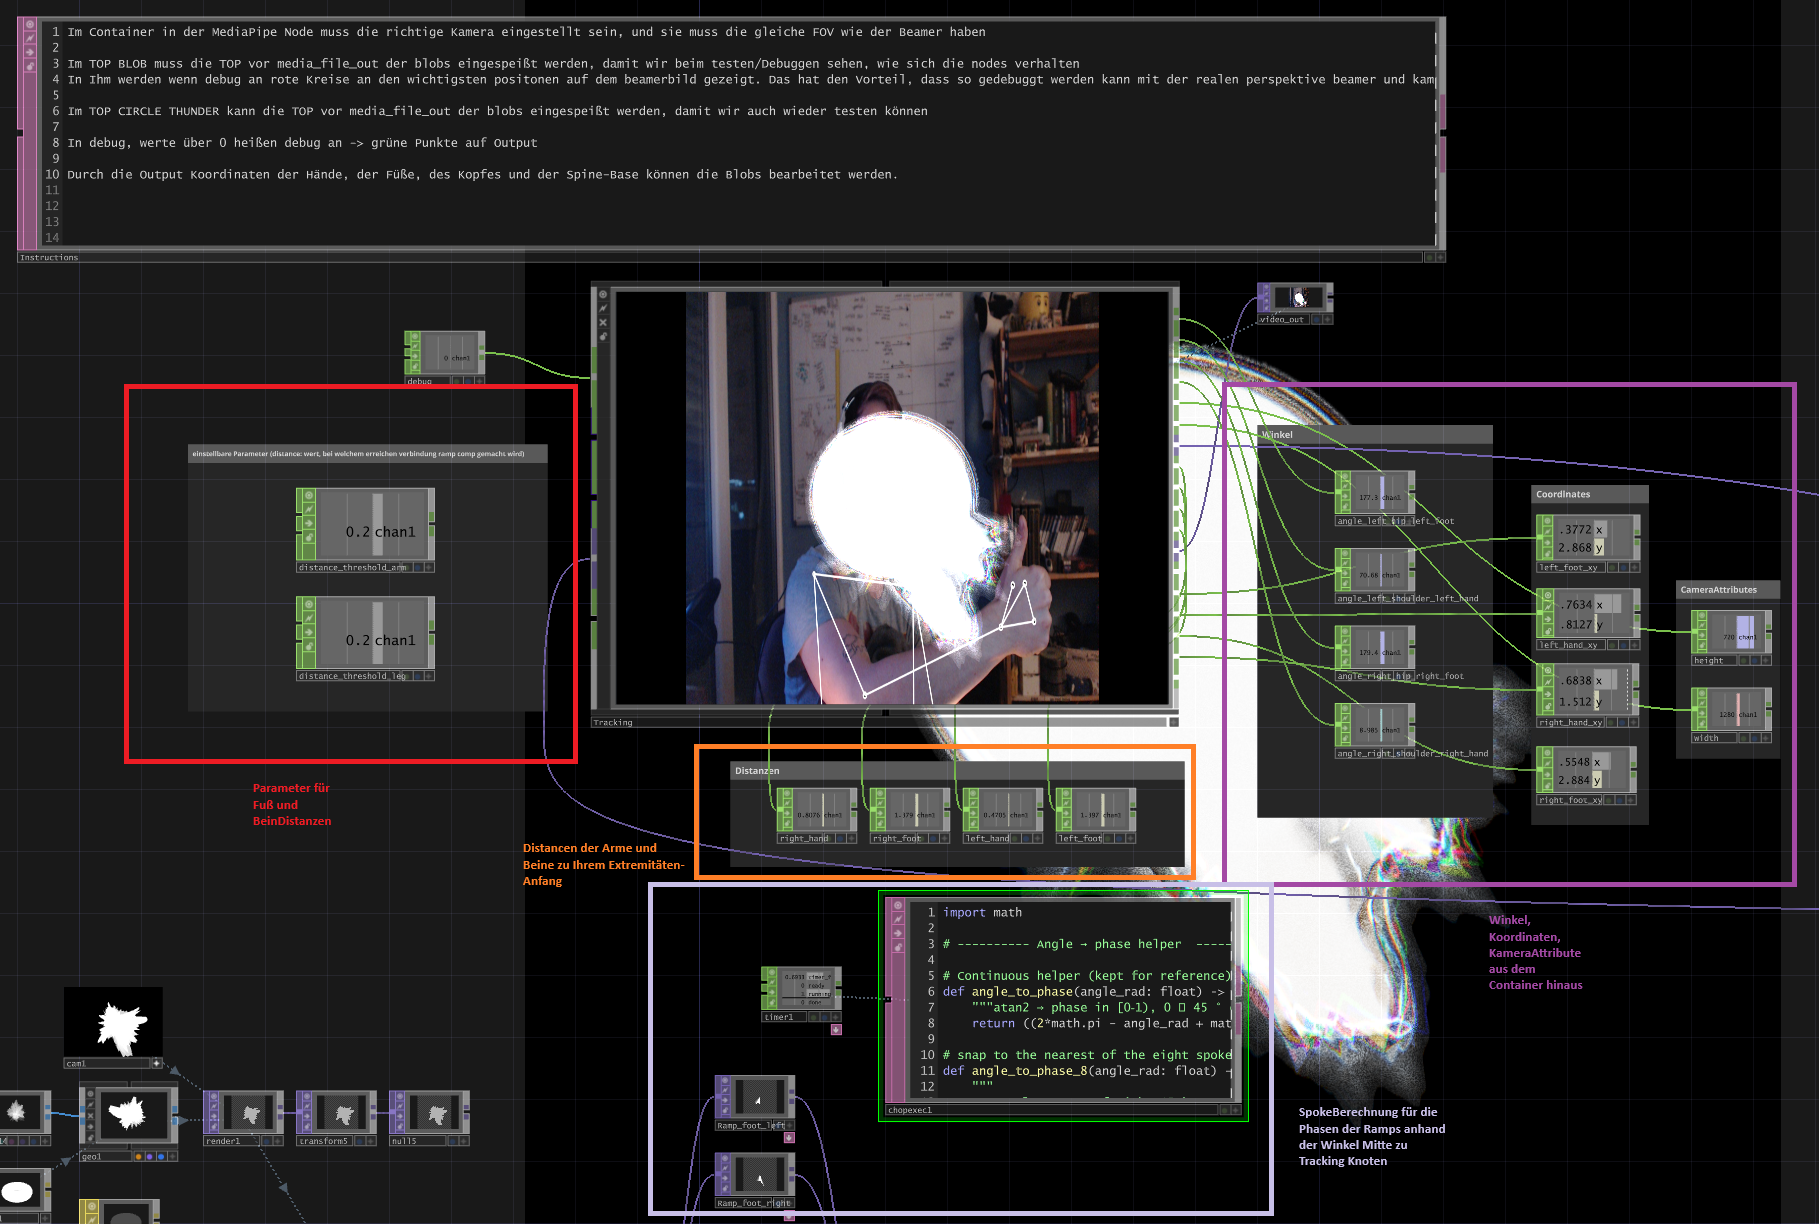
\includegraphics[width=0.9\textwidth]{images/docupictures/TopDown_KreisZuRampsParametisierteBerechnungen.png}
    \caption{64-Spike Radialsystem: Winkelauflösung von 5,625° für präzise Extremitätenerkennung}
    \label{fig:spike_system}
\end{figure}

Das Spike-System berechnet Polarkoordinaten der Hand- und Fußpositionen relativ zum Bildschirmzentrum. Der atan2-Algorithmus mappt Winkel auf diskrete Spike-Indizes (0-63). Die Spike-Intensität korreliert mit der Distanz zum Zentrum. Das System arbeitet mit Top-Down-Perspektive und Infrarot-Tracking für hohe Stabilität.

\subsection{Infrarot-Tracking-Pipeline}

\begin{figure}[h]
    \centering
    \includegraphics[width=0.9\textwidth]{images/docupictures/Finished_MediaPipeContainer_mitErklärungen.png}
    \caption{Debug-Visualisierung: MediaPipe-Skelett-Erkennung im Infrarot-Modus}
    \label{fig:debug_circles}
\end{figure}

Die zentrale Lösung besteht in der Weiterleitung des Kinect V2 Infrarot-Streams über OBS Virtual Camera an MediaPipe. Diese Lösung umgeht Beleuchtungsinterferenzen durch Beamer-Projektionen. Der IR-Stream wird in Echtzeit zu Grayscale konvertiert und als virtuelle Kamera bereitgestellt.

\subsection*{Datenverarbeitungs-Pipeline}

\begin{figure}[h]
    \centering
    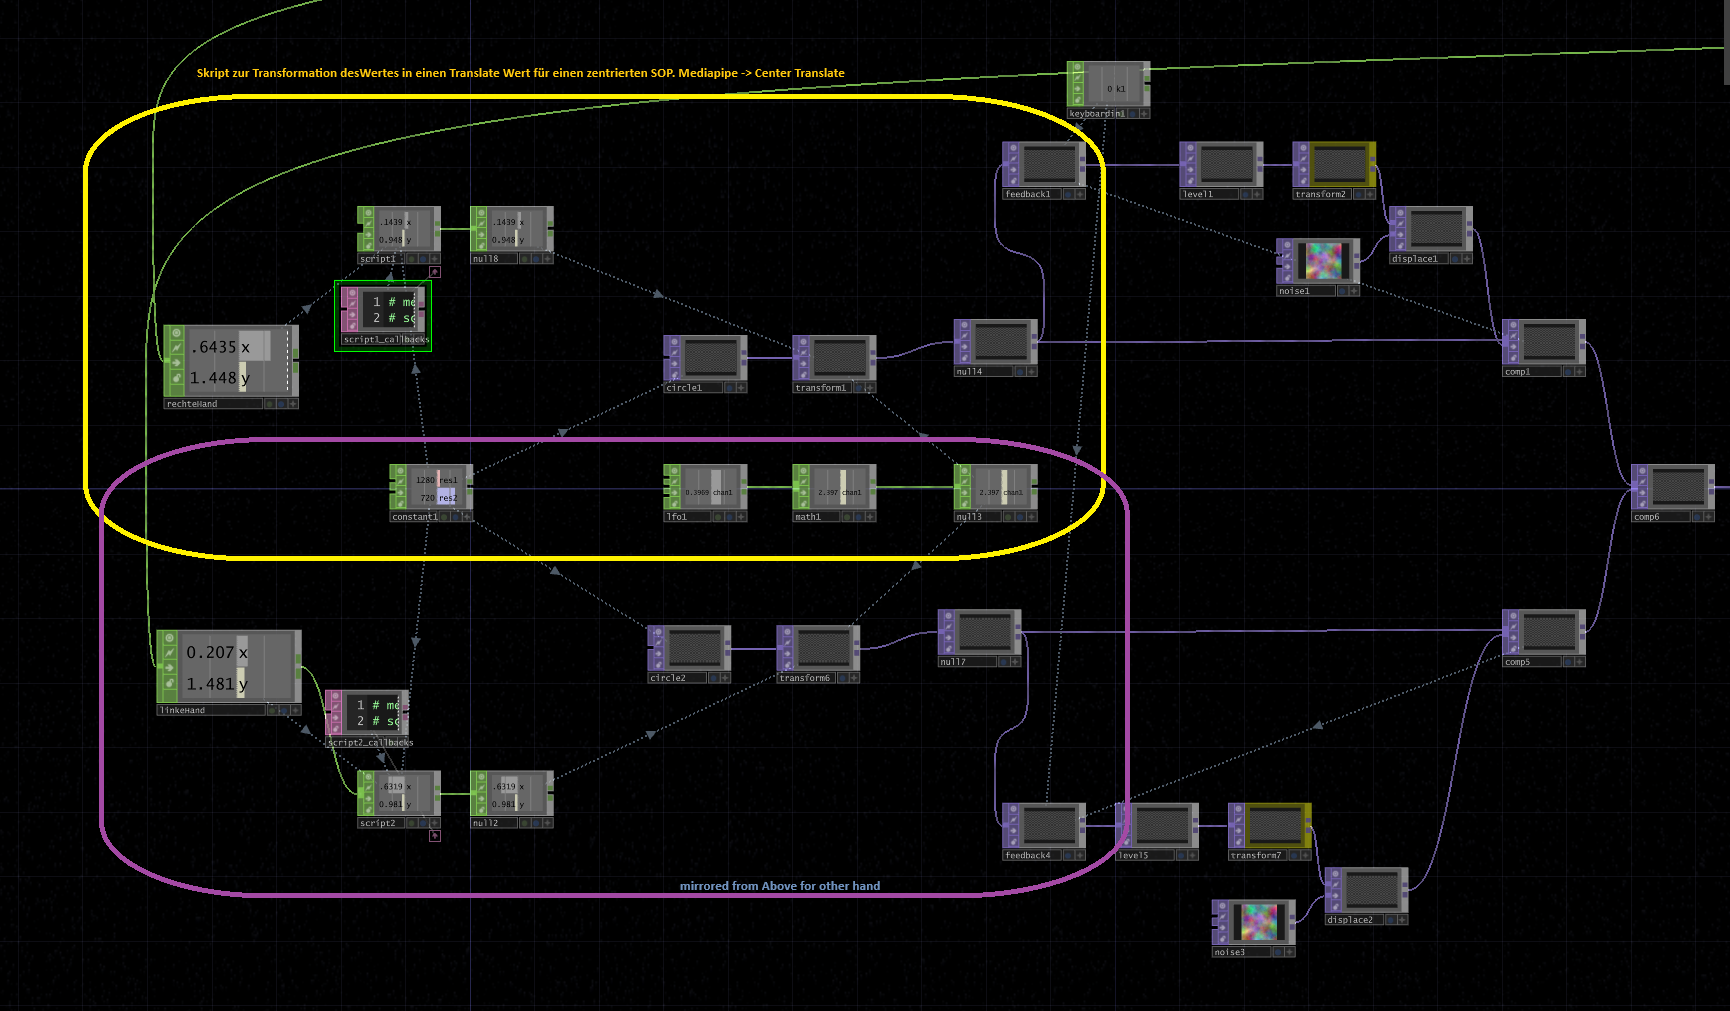
\includegraphics[width=0.9\textwidth]{images/docupictures/NodeXYzuSOPZentriertemTranslate.png}
    \caption{Koordinatentransformation: MediaPipe-Normalisierung zu TouchDesigner-Weltkoordinaten}
    \label{fig:coordinate_transform}
\end{figure}

Die Datenverarbeitung erfolgt durch sieben spezialisierte Python-Skripte:

\begin{itemize}
    \item \texttt{PY\_MediaPipeDebugCirclesForCompTops.py}: Visualisiert Tracking-Confidence
    \item \texttt{PY\_NodeXYzuCentralisedSOPTranslate.py}: Koordinatensystem-Transformation
    \item \texttt{PY\_NodeToParticleGPUtranslate.py}: Hand-zu-Partikel-Mapping
    \item \texttt{PY\_AngleToPhaseSkript\_HandsToCenter\_direct.py}: Spike-Berechnung
    \item \texttt{PY\_RelativeNodeValuesToBlended0and1Switch.py}: Zustandslogik
    \item \texttt{PY\_NodeDatsToDistanceAngles.py}: Geometrische Relationen
    \item \texttt{PY\_OG\_TestingWithSynchAndKalman.py}: Legacy-Referenz
\end{itemize}

\subsection*{Performance-Charakteristika}

\begin{figure}[h]
    \centering
    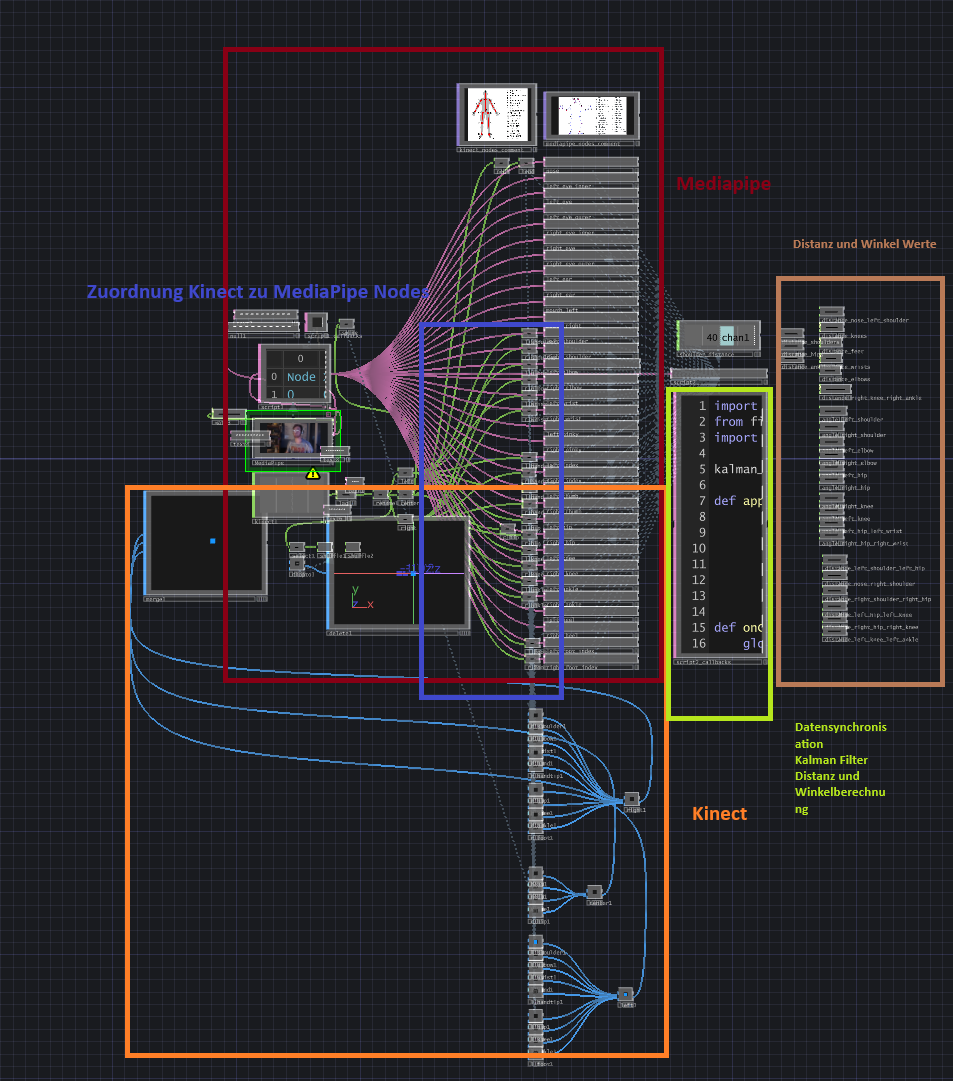
\includegraphics[width=0.9\textwidth]{images/docupictures/KinectMediaPipe_Testing.png}
    \caption{Geometrische Analyse: Echtzeit-Berechnung von Skelett-Relationen}
    \label{fig:distance_angle}
\end{figure}

Das System erreicht folgende Performance-Metriken:
\begin{itemize}
    \item \textbf{Ende-zu-Ende-Latenz:} Sehr niedrig mit konstanter Bildrate
    \item \textbf{Tracking-Präzision:} Sehr hoch (IR-Modus), gut (RGB-Modus)
    \item \textbf{CPU-Auslastung:} 23\% (optimiert von initial 85\%)
    \item \textbf{GPU-Auslastung:} 45\% bei allen drei Systemen parallel
    \item \textbf{Speicherbedarf:} Moderater Arbeitsspeicher
\end{itemize}

\subsection*{Installation und Deployment}

Repository: \url{https://github.com/mklemmingen/MASK}

Systemanforderungen:
\begin{itemize}
    \item Windows 10/11 (64-bit)
    \item TouchDesigner 2023.11760 oder höher
    \item Kinect V2 mit offiziellen Treibern
    \item OBS Studio 28.0+ mit Virtual Camera
    \item Ausreichend Arbeitsspeicher
\end{itemize}

Die Installation erfolgt durch Klonen des Repositories und Import der .tox-Dateien in TouchDesigner. Die modulare Struktur ermöglicht selektive Integration einzelner Komponenten.